\documentclass[../main.tex]{subfiles}

\begin{document}

IOTA's vision aims to establish a real-time economy for Internet-of-Things and the future Internet through a secure zero fee payment and data transmission system.
Realizing this vision is subject to a combination of features that cannot be found in current distributed ledger technologies (DLTs): First, it is required significantly higher throughput than blockchains which have an intrinsic bottleneck forcing transactions to be aggregated under a chain-type data structure; second, fees can be considered a barrier for micro transactions, but they are necessary in PoW-based DLTs where the network distinguishes between miners and users.
Conversely, IOTA utilizes a directed acyclic graph (DAG) structure as explained in the IOTA white paper~\cite{popov2018} which permits a theoretical infinite throughput\footnote{The actual throughput is bounded by hardware limitations and by law of physics.}. Furthermore, enabling each network participant to both issue and approve transactions allows IOTA to eliminate the fees found in blockchain architecture, thus facilitating a micropayment-ready network (see also \cite{popov2019feelessfree}).

%As explained in the IOTA white paper~\cite{popov2018}, IOTA utilizes a directed acyclic graph (DAG) structure to permit a homogeneous network environment. Indeed, without miners who form blocks, the \enquote{pure} blockchain structure is no longer possible in practice, because of network propagation delays; therefore, we naturally arrive to a more general DAG structure. Enabling each network participant to both issue and approve transactions allows IOTA to eliminate the fees found in blockchain architecture, thus facilitating a micropayment-ready network (see also \cite{popov2019feelessfree}). 

One common problem for early stage DLTs is that the networks are not robust enough for proposed security mechanisms to function as intended, since such security mechanisms presuppose a mature network. Therefore, it is typical that DLTs employ various ``bootstrapping'' security measures at the outset, ensuring network growth to the mature stage can take place\footnote{For example, Bitcoin has in the past employed checkpoints. See \url{https://en.bitcoin.it/wiki/Checkpoint_Lockin}}. Thus, in its current implementation, IOTA relies on a centralized Coordinator to provide security given the risk of dishonest actors seeking to undermine the nascent network. IOTA's definition of consensus requires a confirmed transaction to be referenced (either directly or indirectly) by a signed transaction issued by the Coordinator. In other words, the Coordinator can be thought of as a ``finality device''.

We believe that the vision of cryptocurrency networks based on Nakamoto consensus can be improved upon by changing the key underlying assumption about those controlling the majority of the network's hashing power being considered \enquote{honest} by definition (the ``longest chain wins'' rule). In IOTA, the requirement for honest actors to control a majority of the network's hashing power is currently replaced by the use of the Coordinator. The Coordinator is a temporary measure as the IOTA network develops beyond Nakamoto's vision for network consensus.
The Coordicide project is focused on the removal of the Coordinator through the implementation of several network components, as discussed in this working paper. 
%The additional network components discussed in this paper are necessary to achieve the goal of switching off the Coordinator, while ensuring consistency between distinct ledgers.
Despite these additional components, all existing fundamental design features of the Tangle remain in-place.
%Therefore, the introduction of such additional network components represents the natural evolution of IOTA.

In line with the IOTA Foundation's charter as a non-profit organization, our goals as a research department include transparency, collaboration, and community engagement. We aim to open our research work in order to obtain feedback from academia as well as the broad community of enthusiasts. One note of caution, however, is in order: Since our research is highly dynamic in nature, proposed ideas need to be simulated and tested in order to develop specific network components which we feel confident to deploy on the main network. We stress that some of the ideas presented here are works in progress and as such are not fully fleshed out. They are therefore likely to be modified as we make progress and perform simulations. 

\begin{figure}
     \centering
     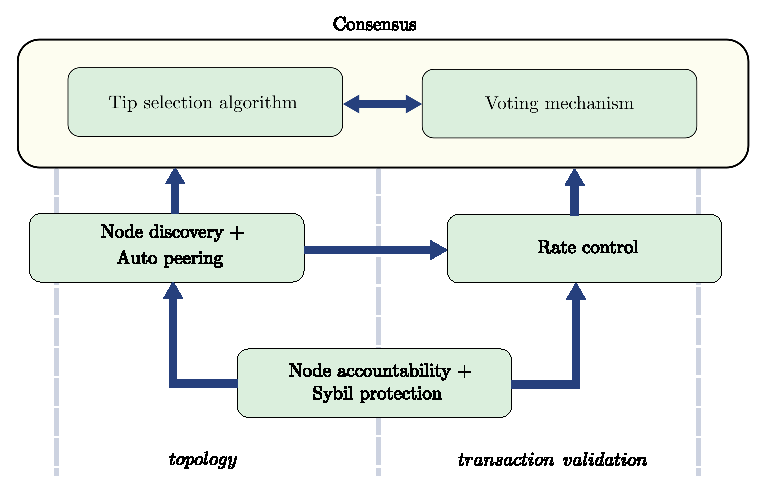
\includegraphics[scale=0.8]{images/building-blocks.eps}
     \caption{Interconnection between the Coordicide building blocks.}
     \label{fig:building-blocks}
\end{figure}

On a high level, our vision for the Coordicide can be explained in the following way. 
We are looking for a \emph{probabilistic consensus} --- with probability very close to $1$, all honest participants of the network would agree on which transactions should be considered valid.
%(``exponential beats polynomial'' magic,
%$n^Me^{-\alpha n}\to 0$). 
It is important to remark that one shouldn't be afraid of the probabilistic nature of it --- if something occurs with strictly
positive probability, this doesn't yet mean it would ever occur 
\emph{in practice}\footnote{as a quick example,
try guessing at least one private key from Bitcoin addresses which belong to Satoshi; yet, the probability that a random 256-bit number is
one of those private keys is strictly positive}.
Another important idea is that, while we do need \emph{total} consensus 
on what is really important (transactions' validity),we may not need total consensus on everything. Therefore, we may
use an \emph{approximate} consensus \footnote{for example, on \emph{time} 
--- it is something on which the approximate consensus already exists; another example when the total consensus is not necessary is the common sequence of random numbers: as explained below, it is already enough if most of the participants agree on the same number frequently enough} 
to achieve the total one with high probability. 
It is also a feature of our approach that the consensus (on transactions' validity) is an \emph{attracting state} in the following sense: small deviations from the absolute consensus on secondary things (e.g., local clocks, random number sequence that the nodes see, mana vectors) with high probability do not lead to deviations from the total consensus on transactions' validity. 
Still, we keep the basic protocol simple: the only ``hard'' rule remains to be that a new transaction should approve two other transactions; 
what eventually stays in the main tangle (not orphaned), 
is valid\footnote{one of the reasons why we prefer using this approach, 
is the following:
if we allow conflicting transactions on the Tangle, 
 this has to go coupled with a precise conflict-resolution rule, 
 which can be never changed and likely has ``long-range'' dependencies''}.
The above in line with the idea that ``IOTA is free'' \cite{popov2019feelessfree}. 
This is because the actors will have flexibility to adapt the system to different environments by only adjusting the node's behaviors.


In order to get rid of the Coordinator, a number of challenges must be solved. This working paper covers those challenges, which are summed up by the building blocks in Fig.~\ref{fig:building-blocks}. In the following, we give a concise overview about the current state of the Coordicide as well as future research directions:
\begin{itemize}
    \item \textit{Node accountability}. In Section~\ref{sec:node_acc} we propose the concept of \emph{global node IDs} and we describe a novel Sybil protection mechanism that does not require node owners to risk or disclose their funds. Identifying the issuing node of a message is fundamental to enforce a specific network topology (through auto peering) or to penalize bad behaviours (through rate control).
    
    \item \textit{Auto peering and node discovery}. 
    An automated process to discover and reliably connect to neighbors is needed in every distributed system. In Section~\ref{sec:peering} we discuss an auto peering proposal for the Tangle.

    \item \textit{Rate control}.
    To ensure the network does not exceed its capacity, in Section~\ref{sec:rate_control} we introduce a mechanism to control the rate of transactions that are propagated through the network. This method selectively filters some transactions out according to the statistics of the issuing node.
    
    \item \textit{Consensus}.
    The previous building blocks lead to an extended consensus framework described in Section~\ref{sec:consensus}. This is made up of two complementary building blocks: First, we describe the current status of research on tip selection algorithms (Section~\ref{sec:tsa}); then, to proactively resolve certain conflicts, we describe two voting mechanisms where nodes query other nodes to find out their current opinion on the network status (Section~\ref{sec:voting}).
\end{itemize}

\end{document}
